\chapter{An Implicit Probabilistic Generative Model}
\label{chapter8}
\graphicspath{{source/chapter8/}}
In previous chapters, we discussed learning in both undirected (Chapter~\ref{chpt5:undirecteLearning}) and directed (Chapter~\ref{chpt6:em-flow} and \ref{chpt7:genhmm}) graphical models. The model learning of previous discussions has been mainly under the principle of maximum likelihood, which includes the cases of MRF learning with approximate inference and the likelihood variational lower bound such as \eqref{chpt5:eq:lower-bound-F}. With maximum likelihood learning, if exactly likelihood is not available, its variational or approximate value is used as the objective function.

In this chapter, we introduce a way of learning a generative model that does not use maximum likelihood. Different from distributions induced by normalizing flows in previous chapters, we do not require the induced distribution $p(\bm{x};\bm{\theta})$ by a generator in the generative model to be tractable here. In another word, the generator-induced distribution $p(\bm{x};\bm{\theta})$ is \textit{implicit} and likelihood-intractable. This relaxation indeed gives us larger freedom of defining the generators since we do not track the Jacobian computation anymore, and thus enlarges the hypothesis space of the model distribution $p(\bm{x};\bm{\theta})$. But it also brings the question of how to learn such a model without the tractable density function. Perhaps, a question before the \textit{how} is the \textit{why}, i.e., why do we need such kind of models?

The motivation for studying these generative models lies in the applications where sampling from implicit distributions is more important than likelihood tractability. Due to the curse of dimensionality, deep generative models that defined with neural network based generators and induce implicit distributions, demonstrate their advantage in the efficiency of modeling complex distributions and sampling in high-dimensional space, in comparison with explicit statistic models. This allows the representation and manipulation of implicitly high-dimensional distributions via the generative models. For instance, deep generative models have been used in image super-resolution, image-to-image translation, etc. Besides, implicit generative models can be naturally incorporated in reinforcement learning where typically an agent tries to learn to finish some tasks via interacting with a dynamic environment. For instance, in model-based methods, using a generative model to represent the environment and generating states for the agent to learn with, offers the way of training agents in simulations; A policy, essentially a conditional distribution of actions given an environment state, may be modeled by an implicit generative model since we mainly need to get the action in the present environment.

In this chapter, we introduce the learning of implicit probabilistic generative models by employing \textit{optimal transport} from transportation theory that does not need the tractability of likelihood. As long as we can simple for a generative model efficiently, learning of the generative model can be formed as the minimization of an optimal transport distance between the induced implicit distribution and an empirical distribution.

\section{Optimal Transport}\label{chpt:sec:ot}
Optimal transport (OT) is a geometric tool for comparison of probability distributions, which has a rich history. Its work traces back as early as $18$th century in Monge's work \cite{monge1781memoire}. OT has been widely used in different fields, such as economic problems, logistics, production planning, etc. Along with its development in history, OT has been given different names, such as earth mover distance, Kantovich distance, and Wasserstein distance. Abstractly, OT distance measures the minimum transportation cost of from the mass of a distribution to another distribution \cite{villani2003topics}. Due to its close relation to the comparison of probability distributions and optimization, OT and its
variants have also been popularly used in machine learning and gained fast development in both theory and applications \cite{2013arXiv1310.4375C, 2013arXiv1306.0895C, 2016arXiv161006519S, ClaiciCS18}.

The high-level idea of this chapter is to use the OT distance to guide us to find the distribution $p(\bm{x}; \bm{\theta})$ of a generative model to approximate the true distribution $p^{\ast}(\bm{x})$. We begin with the introduction to OT itself and make connections to some popular generative models.

We denote the space $(\bm{\Xx},\|\cdot\|_2)$ be our working space, where $\bm{\Xx} = \prod_{x=1}^{N} \Xx_i$ as defined in Chapter~\ref{chapter2}. $\|\cdot\|_2$ is the Euclidean distance. Assume that $\bm{\Xx}_1$, $\bm{X}_2$ are finite sample subsets of $\bm{X}$. Let $p^{\ast}(\bm{x})$ be a distribution on $\bm{\Xx}_1$ and $p(\bm{x};\bm{\theta})$ be a distribution on $\bm{\Xx}_2$.
With mild abuse of notation, we denote the OT distance between $p^{\ast}(\bm{x})$ and $p(\bm{x}; \bm{\theta})$ by $T(p^{\ast},p)$. According to Kantovich's transportation problem\cite{villani2003topics}, we have $T(p^{\ast},p)$ given by
\begin{equation}\label{chpt8:eq:ot}
  T(p^{\ast}, p) = \min_{\pi\in\Pi(p^{\ast}, p)}\langle\pi,\bm{M}\rangle,
\end{equation}
where $\dotp{\cdot}{\cdot}$ stands for the inner product of
two matrices, and $\Pi(p^{\ast},p)$ is a set of joint distribution $\pi$ on
the sample sets $\bm{\Xx}_1\times\bm{\Xx}_2$ such that $\pi$ has
marginal distributions $p^{\ast}(\bm{x})$ and $p(\bm{x}; \bm{\theta})$. 
The cost matrix $\bm{M}$ has elements $M_{i,j} = d(\bm{x}_1^{i}, \bm{x}_2^{j})$ with $d(\cdot, \cdot)$ as a distance (Euclidean distance is used in our implementation), where $\bm{x}_1^{i}\in\bm{\Xx}_1$ and $\bm{x}_2^{j}\in \bm{\Xx}_2$ are $i$th and $j$th samples from $p^{\ast}(\bm{x})$ and $p(\bm{x}; \bm{\theta})$, respectively. 


\begin{remark}[Connection to the vanilla generative adversarial network]
  In the model learning of previous chapters, the information on how the model should adjust (change its parameter) is given by the likelihood value, stemming from KL divergence. In this chapter, we introduce the OT distance to offer such information in modeling learning. There are other ways to achieve this goal. A popular one is the generative adversarial network (GAN) \cite{NIPS2014_5423, 2017arXiv170100160G}, which casts the generative model learning into an adversarial game between the generator $\bm{g}$ and a discriminator $f$.
The {discriminator} $f$ gets input from either output of $\bm{g}$ or from
$p^{\ast}$. The generator $\bm{g}$ and discriminator ${f}$ play against each other
regarding a min-max objective:
\begin{equation}\label{chpt8:eq:eq-gan}
  \min_{\bm{g}} \max_f \EE_{p^{\ast}(\bm{x})}\left[ \log(f(\bm{x})) \right] + \EE_{p(\bm{z})}\left[ \log(1-f(\bm{g}(\bm{z})) \right],
\end{equation}
where $p(\bm{z})$ is a fixed distribution and easy to sample from. The model distribution $p(\bm{x}; \bm{\theta})$ is an implicit distribution and is induced by $\bm{x} = \bm{g}(\bm{z})$.
The probability model learning relies on if min-max game finds
its equilibrium where distribution $p(\bm{x}; \bm{\theta})$ is the same as $p^{\ast}(\bm{x})$ and
$d$ is optimal. In optimal case of the discriminator, objective of
\eqref{chpt8:eq:eq-gan} is to minimize the Jensen-Shannon divergence between $p(\bm{x}; \bm{\theta})$ and $p^{\ast}(\bm{x})$.
\end{remark}


\begin{remark}[Connection to Wassertein GAN]\label{chpt8:rmk:wgan}
  It is interesting to note that the OT minimization can be connected to GANs via its duality form. According to Kantorovich-Rubinstein duality \cite[section~2.4]{2018arXiv180300567P}\cite{villani2008optimal},
  \begin{equation}\label{chpt8:eq:kr-duality}
     T(p^{\ast},p) = \sup_{\|f\|_{L} \leq 1} \EE_{p^{\ast}(\bm{x})}\left[ f(\bm{x}) \right] -
  \EE_{p(\bm{x};\bm{\theta})}\left[ f(\bm{x}) \right],
\end{equation}
$\|f\|_L$ is a constraint for $f$ such that $f$ belong to the 1-Lipschitz function
family. That is to say, $f$ in \eqref{chpt8:eq:kr-duality} can be any function from the 1-Lipschitz function
family (which is different from the binary discriminator in \eqref{chpt8:eq:eq-gan}). Then minimization of the OT distance is formulated as a min-max problem \cite{2017arXiv170107875A}, termed as Wasserstein GAN (WGAN),
\begin{equation}\label{chpt8:eq:eq-wgan}
  \min_{\bm{g}} \max_{\|f\|_{L} \leq 1} \EE_{\bm{x} \sim p^{\ast}(\bm{x})}\left[ f(\bm{x}) \right] -
  \EE_{\bm{z}\sim p(\bm{z})}\left[ f(\bm{g}(\bm{z})) \right],
\end{equation}
where $p(\bm{x};\bm{\theta}) = p(\bm{g}(\bm{z}); \bm{\theta})$ with $\bm{\theta}$ parameterizing $\bm{g}$ and $\bm{z}\sim p(\bm{z})$. The  Lipschitz constraint enforcing is not trivial in general, especially for the deep generative models where $\bm{g}$ is implemented by neural networks. Nevertheless, the vanilla GAN in \eqref{chpt8:eq:eq-gan} is similar to the \eqref{chpt8:eq:eq-wgan} from minimization of OT distance.
\end{remark}

\begin{remark}[Connection to auto-encoders]
It is known that the variational lower bound of the likelihood function as in \eqref{chpt5:eq:lower-bound-F} is used to train variational auto-encoders, where an encoder and a decoder adjust their parameters to maximize the variational lower bound in the maximum likelihood principle. Since OT offers an alternative tool for modeling learning, it is also employed to train auto-encoders in likelihood-free settings, which shares similarities with the variational auto-encoders. See \cite{patrini2018sinkhornVAE, genevay2017gan,bousquet2017optimal} for detailed discussions.
\end{remark}

\section{EOT based Generative Models}

The optimal transport problem in \eqref{chpt8:eq:ot} is highly intractable. Therefore, approximation has to been used for efficient solutions. In Remark~\ref{chpt8:rmk:wgan}, Kantorovich-Rubinstein duality offers one way to solve the problem in its dual form if the Lipschitz constraint can be properly enforced. An alternative way can be using entropy regulation to seek for \textit{soft} solution.  In this section, we introduce the entropy-regularized optimal transport (EOT) cost and then propose generative models accordingly.

\subsection{Entropy-regularized OT} 

OT calculates the minimum cost of transporting distribution $p^{\ast}(\bm{x})$ to $p(\bm{x}; \bm{\theta})$. We use $W(p^{\ast},p)$ to denote entropy-regularized OT (EOT) cost as follows:
\begin{equation}\label{eq-entropic-wsd}
  W(p^{\ast},p)=\min_{ \pi \in \Pi(p^{\ast}, p)} \dotp{\pi}{\bm{M}} - \la H(\pi),
\end{equation}
where $H(\pi)$ is the entropy of joint distribution $\pi$, i.e. $H(\pi) = \sum_{i,j} -\pi_{i,j}
\log(\pi_{i,j})$ and $\la \in \RR_{+}$ is the regularization
parameter. Here $\RR_{+}$ denotes positive scalars. The entropy regularization in \eqref{eq-entropic-wsd}  translates 
to a requirement that the joint distribution $\pi$ has a high entropy. 
 The duality of EOT cost in \eqref{eq-entropic-wsd} is
\begin{equation}\label{eq-dual-wsd}
  W(p^{\ast}, p)  =  \max_{\bm{\al}, \bm{\be} \in \mathbb{R}^{N}} \bm{\al}^{\intercal}p^{\ast} + \bm{\beta}^{\intercal}p \! - \!
  \sum_{i,j} \lambda e^{ \frac{{\left( \al_i + \beta_j - M_{i,j} \right)}}{\la} },\vspace{-2pt}
\end{equation}
where $\bm{\alpha},\bm{\beta}$ are dual variables, $(\cdot)^{\intercal}$ means transpose, $\alpha_i$ is the $i$th element of $\bm{\alpha}$, and $\beta_i$ is the $j$th element of $\bm{\beta}$

One benefit of having the dual variables is that the optimal dual vector $\bm{\beta}^{\ast}$
of \eqref{eq-dual-wsd} is a subgradient of $W(p^{\ast},p)$ with respect to $p$. Thus, if we can efficiently obtain the optimal dual vector $\bm{\beta}^{\ast}$, we can learning our model distribution $p(\bm{x}; \bm{\theta})$ via the subgradient $\bm{\beta}^{\ast}$.

There is a computationally efficient algorithm called Sinkhorn
algorithm\cite{2013arXiv1306.0895C, 2013arXiv1310.4375C} to
solve~\eqref{eq-dual-wsd}, which alternatively scales the rows and columns of matrix $e^{-\frac{\bm{M}}{\lambda}}$. This alternative computation gives a pair of vectors $(\bm{u}, \bm{v}) \in \RR^N_{+} \times \RR^N_{+}$ that defines the optimal primary and dual variavles \cite[Proposition~2]{2013arXiv1310.4375C} 
\begin{align}\label{eq-dual-opt}
  \pi^{\ast} &=
               \mathrm{diag}(\bm{u}) \, e^{\frac{-\bm{M}}{\la}} \, \mathrm{diag}(\bm{v}),  \nonumber \\
  \bm{\beta}^{\ast} &= \frac{\log(\bm{u}^{\intercal})\mathds{1}_N}{N\la} \mathds{1}_N -\frac{\log(\bm{u})}{\la}.
\end{align}
where $\mathrm{diag}(\bm{u})$ is a matrix with diagonal entries from vector $\bm{u}$ and $\mathds{1}_N$ is a column vector with ones.


\subsection{EOT based Generative Models}

In this subsection, we propose two generative models.
We first develop an EOT based generative model handling signals/data directly. This models is referred to as EOT generative model (EOTGM). 
In our second model, we use a
representation mapping where EOT cost is used to optimize the
generative model and representation mapping jointly. The second model is referred as EOT based GAN (EOTGAN).
% In our EOT based GAN, we have a generator, but do not have an explicit discriminator. Instead we use a representation mapping where EOT cost is used to optimize the generator function and representation function jointly. We first develop an EOT based algorithm for generative model learning that can handle signals/data directly. Then we develop second algorithm that can handle representation features. The second algorithm is referred to as EOT based GAN (EOTGAN). 

\subsubsection{EOT based generative model (EOTGM)}\label{subsec-gmeot}
{Although the true probability distribution $p^{\ast}(\bm{x})$ is not available but its empirical distribution is available, i.e. the dataset. We carry on using the notation $p^{\ast}(\bm{x})$ as the target distribution. $p(\bm{x};\bm{\theta})$ is the probability distribution of our model induced by a generator $\bm{g}: \bm{\Zz} \rightarrow \bm{\Xx}$, where $\bm{\Zz}$ is the support set of latent distribution $p(\bm{z})$. The generator $\bm{g}$ is implemented by a neural network and maps latent signal $\bm{z} \in \bm{\Zz}$ to signal in $\bm{\Xx}$, i.e., $\bm{g}(\bm{z}) \in \bm{\Xx}$. The latent distribution is assumed to be known. The mapped signal $\bm{g}(\bm{z}) \sim p(\bm{x};\bm{\theta})$ since $\bm{g}$ induces the model distribution. Actually, the parameter of $p(\bm{x};\bm{\theta})$ is the parameter of the generator $\bm{g}$. Applying EOT cost to learn $p(\bm{x}; \bm{\theta})$ is equivalent to minimizing $W(p^{\ast}, p)$ w.r.t. the generator $g$}
\begin{equation}\label{eq-entropic-model}
  \underset{\bm{g}:\bm{\mathcal{Z}}\to \bm{\Xx}}{\argmin}\, W(p^{\ast}, p) = \underset{\bm{\theta}}{\argmin}\, W(p^{\ast}, p).
\end{equation}
Since $\bm{\beta}^{\ast}$ in \eqref{eq-dual-opt} is subgradient of $W(p^{\ast}, p)$ w.r.t. $p(\bm{x};\bm{\theta})$, we are able to
optimize the generator $\bm{g}$ such that the induced distribution $p(\bm{x};\bm{\theta})$ approximates $p^{\ast}(\bm{x})$, using gradient chain rule gives
\begin{equation}
  \nabla_{\bm{\theta}}W(p^{\ast}, p) = \left(\nabla_{\bm{\theta}}p\right)^{T} \bm{\beta}^{\ast}.
\end{equation}
Alternatively the optimization problem \eqref{eq-entropic-model} can be addressed by solving $\argmin_{g}\dotp{\pi^{\ast}}{\bm{M}} $ iteratively using auto-gradient functions in PyTorch\cite{pytorch} or
TensorFlow\cite{tensorflow}, where $\pi^{\ast}$ is primary optimal
variable to \eqref{eq-entropic-wsd} given by \eqref{eq-dual-opt}. We
propose Algorithm~\ref{algo-E-WL} to learn distribution $p^{\ast}$
via minimizing the EOT loss w.r.t parameter $\bm{\th}$ of generator function $\bm{g}$.
\begin{algorithm}[!t]
  \caption{EOT based Generative Model (EOTGM)}\label{algo-E-WL}
  \begin{algorithmic}[1]
    \STATE{$l$: the update rate at each iteration. $N$: the batch
      size. $\bm{\th}_{0}$: the initial parameter for $\bm{g}$.}
    \WHILE{$\bm{\theta}$ has not converged}
    \STATE Sample  a batch from a real dataset, $\left\{ \bm{x}^{i} \right\}_{i=1}^{N} \sim p^{\ast}$. 
    \STATE Sample $\left\{ \bm{z}^{i} \right\}_{i=1}^{N} \sim p(\bm{z})$, a batch of latent samples.
    \STATE Passing $\left\{ \bm{z}^{i} \right\}_{i=1}^{N}$ through the generator $\bm{g}$.
    \STATE Calculate the cost matrix $M$.
    \STATE $\pi^{\ast}$, $\bm{\beta}^{\ast} \gets$ primary and dual
    solutions of $W(\left\{ \bm{x}^{i} \right\}_{i=1}^{N}, \left\{
      \bm{g}(\bm{z}^{i})\right\}_{i=1}^{N})$ according \eqref{eq-dual-opt}.
    \STATE $\bm{\theta} \gets \bm{\theta} - l \left(\nabla_{\bm{\th}}{p}\right)^{\intercal}
    \bm{\beta}^{\ast}$. (Or back propagate using loss $\dotp{\pi^{\ast}}{\bm{M}}$)
    \ENDWHILE
  \end{algorithmic}
\end{algorithm}

\subsubsection{EOT based GAN (EOTGAN)}

In this section, we consider representation learning (feature
learning) with which the usage of EOT is more meaningful than that
directly in signal space.
It is well-known that Euclidean distance is not well suited to compare
two multimedia signals. For example, Euclidean distance between an
image and its rotated version can be large, but they are visually same. In Algorithm \ref{algo-E-WL} we construct cost matrix $\bm{M}$ in EOT using 
Euclidean distance between real signals and generated signals. Our new proposal is to transform signal through a representation mapping 
$\bm{f}: \bm{\Xx} \rightarrow \bm{\Mm}$, $\bm{\mathcal{M}}\subset\mathbb{R}^{m}$ and we compare features in the representation space via EOT. We assume that Euclidean distance
between features in the representation space is more semantically
meaningful. An element of the cost matrix $\bm{M_f}$ in representation domain (feature domain) is
\begin{equation}\label{def-similarity}
  d_{\bm{f}}(\bm{x}, \bm{y}) = \|\bm{f}(\bm{x})-\bm{f}(\bm{y})\|_{2}.
\end{equation}

Our new objective is joint learning of generator $\bm{g}$ and representation $\bm{f}$. A natural question is how to construct $\bm{f}$ function? {Inspired by the triplet loss in \cite{7298682} aiming at larger distance between distinct classes than in-class distance, we may consider two virtual classes labeled by $p^{\ast}(\bm{x})$ and $p(\bm{x};\bm{\theta})$.
% Then samples from the same class share more similarity and thus should have smaller distance in $\Mm$.
This means that the representation function $\bm{f}$ should have the algebraic property: $ d_{\bm{f}}(\bm{x}_1, \tilde{\bm{x}}_1) + \gamma \leq d_{\bm{f}}(\bm{x}_1, \bm{x}_2) $ for $\gamma > 0$, where $\bm{x}_1, \tilde{\bm{x}}_1 \in \bm{\Xx}_1$ are two samples from distribution $p^{\ast}$ and $\bm{x}_2$ is a generated signal from distribution $p(\bm{x};\bm{\theta})$, i.e., an output of $\bm{g}$. Meanwhile, $\bm{g}$ tries to mitigate this distinction.}

Following the above idea, let us denote the mapped distribution via $\bm{f}$ by $p^{\ast}_{\bm{f}}$ and $p_{\bm{f}}$, respectively. Let $\bm{M}_{\bm{f}}$ be the cost matrix in representation domain and its elements $M_{\bm{f},{i,j}} = d_{\bm{f}}(\bm{x}^{i}_1, \bm{x}^{j}_2)$, $\bm{x}^{i} \sim p^{\ast}(\bm{x}), \bm{x}^{j}\sim p(\bm{x}; \bm{\theta})$. Then we learn $\bm{f}$ and $\bm{g}$ using alternative optimization, as follows. 
\begin{itemize}
\item Learning of representation $f$ is minimizing EOT cost
  \begin{equation}\label{eq-sim-in}
    W(p^{\ast}_{\bm{f}},p^{\ast}_{\bm{f}}) = \min_{\widetilde{\pi} \in \Pi(p^{\ast}_{\bm{f}}, p^{\ast}_{\bm{f}}) } \dotp{\widetilde{\pi}}{\widetilde{\bm{M}}_{\bm{f}}} - \la H(\widetilde{\pi}),
  \end{equation}
  where $\widetilde{M}_{\bm{f}, {i,j}} = d_{\bm{f}}(\bm{x}^{i}, \tilde{\bm{x}}^{j})$, $\bm{x}^{i}, \tilde{\bm{x}}^{j} \sim p^{\ast}(\bm{x})$, and maximizing EOT cost
  \begin{equation}\label{eq-sim-ex}
    W(p^{\ast}_{\bm{f}}, p_{\bm{f}}) = \min_{{\pi} \in \Pi(p^{\ast}_{\bm{f}}, p_{\bm{f}}) } \dotp{{\pi}}{\bm{M_f}} - \la H({\pi}).\vspace{-8pt}
  \end{equation}
\item Learning of generator $\bm{g}$ is minimizing EOT cost
  \begin{equation}
    W(p^{\ast}_{\bm{f}}, p_{\bm{f}}).
  \end{equation}
\end{itemize} 
Both $W(p^{\ast}_{\bm{f}}, p^{\ast}_{\bm{f}})$and $W(p^{\ast}_{\bm{f}}, p_{\bm{f}})$ have lower bounds, but no upper bounds. 
We combine the step 1 in above using a hinge loss and define the following costs.
\begin{equation}
  \begin{array}{rl}
    &\Ll_{\bm{f}}(p^{\ast}_{\bm{f}}, p_{\bm{f}}) := \max\left(0, W(p^{\ast}_{\bm{f}}, p^{\ast}_{\bm{f}})- W(p^{\ast}_{\bm{f}}, p_{\bm{f}}) \hspace{-2pt}+\hspace{-2pt} \gamma \right),\\
    &\Ll_{\bm{g}}(p^{\ast}_{\bm{f}}, p_{\bm{f}}) := W(p^{\ast}_{\bm{f}}, p_{\bm{f}}),
  \end{array}
\end{equation}
where $\gamma>0$. Hinge loss helps to balance the adversarial training of the $\bm{f}$ and $\bm{g}$.
Note the our hinge adversarial loss shares similarity only in form to the self-attention GAN\cite{2018arXiv180508318Z} and geometric GAN\cite{2017arXiv170502894L} but is motivated differently and defined in different metric. We used neural networks for constructing $\bm{f}$ and $\bm{g}$ functions. Let us assume that the parameters of $\bm{f}$ and $\bm{g}$ are $\bm{\omega}$ and $\bm{\theta}$, respectively. Then the adversarial training between representation $\bm{f}$ and
generator $\bm{g}$ is the following alternative optimization problem
\begin{equation}
  \begin{array}{rl}
    &\min_{\bm{f}} \Ll_{\bm{f}}(p^{\ast}_{\bm{f}}, p_{\bm{f}}) = \min_{\bm{\omega}} \Ll_{\bm{f}}(p^{\ast}_{\bm{f}}, p_{\bm{f}}), \\ 
    &\min_{\bm{g}}\Ll_{\bm{g}}(p^{\ast}_{\bm{f}}, p_{\bm{f}}) = \min_{\bm{\th}}\Ll_{\bm{g}}(p^{\ast}_{\bm{f}}, p_{\bm{f}}).
  \end{array}\vspace{-2pt}
\end{equation}
The algorithm steps of EOTGAN are shown in Algorithm \ref{algo-eWGAN}.

\begin{algorithm}[!t]
  \caption{EOT based GAN (EOTGAN)}\label{algo-eWGAN}
  \begin{algorithmic}[1]
    \STATE {$l$: the update rate at each iteration. $N$: the batch
      size. $\bm{\th}_{0}$, $\bm{\omega}_0$: the initial parameters for $\bm{g}$ and $\bm{f}$.}
    \WHILE{$\bm{\theta}$ has not converged}
    \STATE Sample two batches of data $ \left\{ \bm{x}^{i}
    \right\}_{i=1}^{N}, \left\{ \tilde{\bm{x}}^{i} \right\}_{i=1}^{N}  $,
    and latent samples $\left\{ \bm{z}^{i} \right\}_{i=1}^{N} $,
    $\bm{x}^{i},\tilde{\bm{x}}^{i} \sim p^{\ast}(\bm{x}), \bm{z}\sim p(\bm{z})$.
    \STATE Passing
    $\left\{ \bm{z}^{i} \right\}_{i=1}^{N}$ through $\bm{g}$.
    \STATE $\widetilde{\pi}^{\ast} \gets$ solving $ W_{\bm{f}}\left( \left\{ \bm{f}(\bm{x}^{i})
      \right\}_{i=1}^{N} , \left\{ \bm{f}(\tilde{\bm{x}}^{i})
      \right\}_{i=1}^{N}\right)$
    \STATE ${\pi}^{\ast} \gets$ sovling $W_{\bm{f}}\left( \left\{ \bm{f}(\bm{x}^{i})
      \right\}_{i=1}^{N}, \left\{ \bm{f}(\bm{g}(\bm{z}^i))
      \right\}_{i=1}^{N} \right)$
    \STATE $\partial{\bm{f}} \gets \nabla_{\bm{\om}} \max\left(0,  \dotp{\widetilde{\pi}^{\ast}}{\widetilde{\bm{M}}}-\dotp{{\pi^{\ast}}}{\bm{M}}+ \gamma\right)$
    \STATE $\bm{\om} \gets \bm{\om} - l \cdot \partial{\bm{f}}$
    \STATE Sample $\left\{ \bm{z}^{i} \right\}_{i=1}^{N}$
    and get $ \left\{ \bm{g}(\bm{z}^i)\right\}_{i=1}^{N}$ via $\bm{g}$.
    \STATE $\pi^{\ast} \gets$ sovling $W_{\bm{f}}\left( \left\{ \bm{f}(\bm{x}^{i})
      \right\}_{i=1}^{N}, \left\{ \bm{f}(\bm{g}(\bm{z}^{i}))
      \right\}_{i=1}^{N} \right)$
    \STATE $\partial{\bm{g}} \gets \nabla_{\bm{\th}} \dotp{\pi^{\ast}}{\bm{M}}$
    \STATE $\bm{\th} \gets \bm{\th} -l \cdot \partial{\bm{g}}$
    \ENDWHILE
  \end{algorithmic}
\end{algorithm}

\subsubsection{Advantage of EOT against OT}

Usage of entropy regularization in EOT avoids the need for Kantorovich-Rubinstein duality
of OT, thus is free from Lipschitz constraint. In literature, several methods endeavor to
satisfy Lipschitz constraint, for example, projecting neural network
parameters into a space fulfilling Lipschitz constraint via weight
clipping \cite{2017arXiv170107875A}, spectrum
normalization \cite{2018arXiv180205957M}, or adding gradient 
penalty into GAN's cost function \cite{2017arXiv170400028G}. Projecting
approaches bring the problem of neural network capacity underuse and
limit its ability to learn complex mapping. Gradient penalty approach takes
gradients of each layer's weight parameters of a neural network into
GAN's cost, thus computation complexity grows fast as the neural
network goes deeper. 
EOT avoids the above-mentioned problems and also has the benefit of lower
computation complexity. With entropy-regularization and Sinkhorn
algorithm, the computation complexity scales as $\mathcal{O}(N^2)$ \cite{2013arXiv1306.0895C}. 
On the other hand, solving OT cost using interior-point methods has a computational requirement as 
$\mathcal{O}(N^3\log{N})$. 


\section{Experimental Results}
We perform experiments to justify our arguments on loss choice and algorithms. We evaluate our
generative models on a toy synthetic dataset of Gaussian-mixture distribution and real image digit dataset MNIST.
\begin{figure*}[!ht]
  \captionsetup[subfigure]{justification=centering}
  \centering
  \begin{subfigure}[b]{0.44\textwidth}
    \centering
    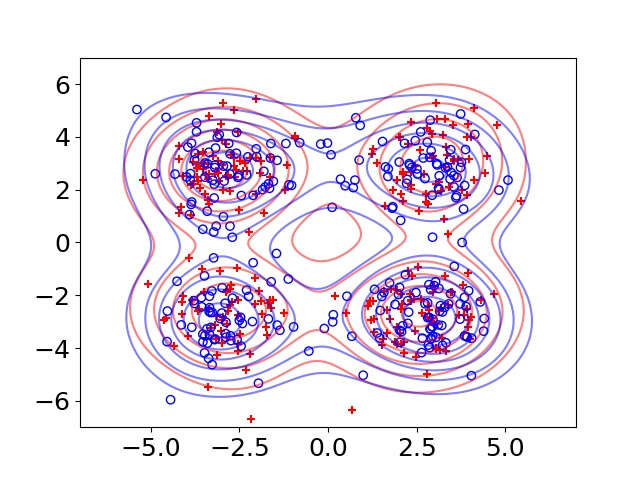
\includegraphics[width=1\linewidth]{images/toy/gauss4/frame8.jpg}
    \caption{}
    \label{fig-toy}
  \end{subfigure}
  \centering
  \begin{subfigure}[b]{0.44\textwidth}
    \centering
    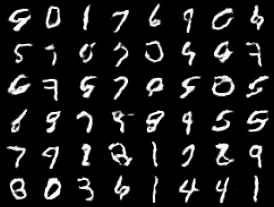
\includegraphics[width=0.8\linewidth]{images/mnist/fake/eot_18500_crop.png}\vspace{5pt}
    \caption{}
    \label{fig-fake-wgan}
  \end{subfigure}
  \centering
  \begin{subfigure}[b]{0.44\textwidth}
    \centering
    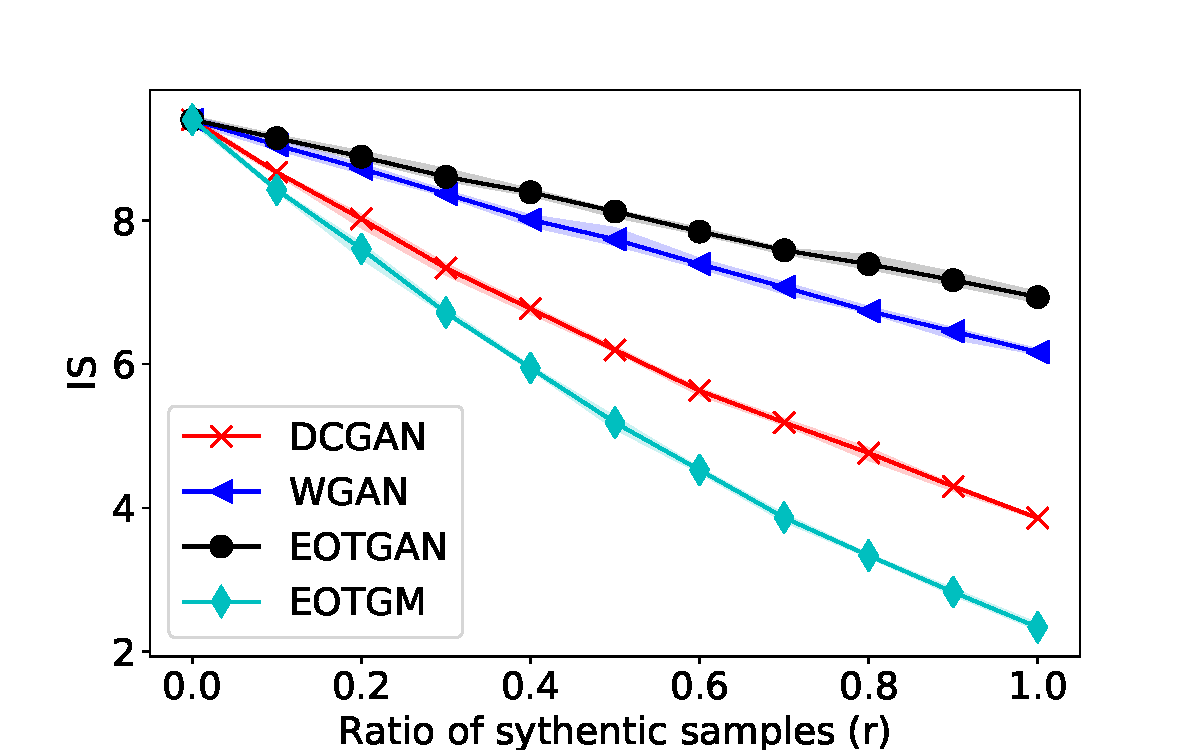
\includegraphics[width=1.1\linewidth]{images/mnist/tra_score/IS_29.pdf}\vspace{-3pt}
    \caption{}
    \label{fig-tra-is}
  \end{subfigure}
  \begin{subfigure}[b]{0.44\textwidth}
    \centering
    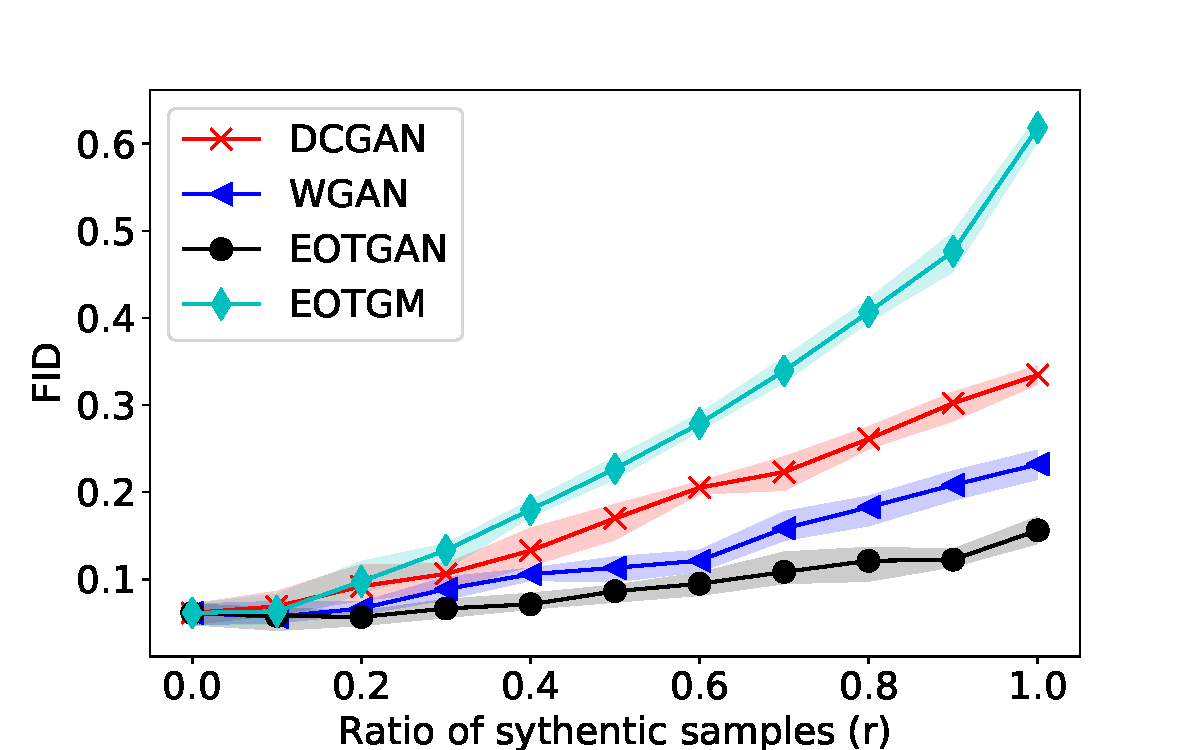
\includegraphics[width=1.1\linewidth]{images/mnist/tra_score/FID_29.pdf}\vspace{-3pt}
    \caption{}
    \label{fig-tra-fid}
  \end{subfigure}
  \caption{(a) Toy distribution learning ($4$-mixture Gaussians) using EOTGM. Real samples (red '+') and contour
    (red curve), versus generated samples (blue 'o') and contour
    (blue curve) by $\bm{g}$. (b) Generated samples by EOTGAN for MNIST dataset. (c) and (d)
    Comparison of IS and FID (on MNIST) versus mixing ratio $r$. (For
    each model at a certain mixture ratio, $5$ experiments are
    independently performed. Each solid curve with markers plots the mean of $5$
    experiments with shaded areas denoting the range of corresponding
    results.}
  \label{fig-tra-score}
\end{figure*}

\subsection{Evaluation Metrics}\label{subsec-metric}
Inception Score (IS) has been popularly used in evaluation of GAN
models\cite{NIPS2016_6125}. IS is defined as $
  IS(q) = \exp\bigl[ \EE_{\bm{x} \sim q} \mathrm{KL}\bigl( p(c | \bm{x})\| p(c) \bigr)  \bigr]$,
where $\bm{x}\sim q$
indicates synthetic sample from distribution $q$ induced by generator $\bm{g}$, $\mathrm{KL}(\cdot, \cdot)$ is Kullback-Leibler divergence, $p(c|\bm{x})$ is the
conditional class distribution, and $p(\bm{x}) = \int_{\bm{x}}p(c|\bm{x}) \,d q(\bm{x})$
is the marginal class distribution. Large IS score means generated
samples contain clear objects. Generative models with high IS can output high
diversity of samples.
Apart from KL-based metric,
an alternative common metric is Frechet Inception Distance (FID)\cite{2017arXiv170608500H}. FID measures the OT distance
of two probability distribution by assuming the two distributions are
Gaussian. Smaller FID means the generated samples are more similar to
empirical samples. Both FID and IS will be used in our experiments. High IS and low FID are better. 

\vspace{-3pt}
\subsection{Evauation of EOTGM using toy dataset}\label{subsec-mg}

{We firstly evaluate our proposed EOTGM on a toy dataset sampled from a known probability
  distribution: two-dimensional four-mixture Gaussian. This mixture Gaussian is our target distribution to learn, i.e., $P$. The generator $\bm{g}$ uses a neural network with structure: Input $\rightarrow$ Dense $256$ $\rightarrow$ ReLU $\rightarrow$ Dense $256$ $\rightarrow$ ReLU $\rightarrow$ Dense $256$ $\rightarrow$ ReLU$\rightarrow$Dense $2$. The parameter $\bm{\theta} $ of $\bm{g}$ here is the set of parameters of this neural network. Latent distribution $p(\bm{z})$ used here is standard Gaussian: $\mathsf{N}\left(\bigl(\begin{smallmatrix}& 0\\
    &0\end{smallmatrix}\bigr) ,\bigl( \begin{smallmatrix}1 & 0\\ 0 &
    1\end{smallmatrix}  \bigr)\right)$.
The toy dataset is used by Algorithm~\autoref{algo-E-WL} (EOTGM) to train $\bm{g}$. In Fig.\ref{fig-toy}, we plot the empirical samples from our toy dataset and the synthetic samples generated by $\bm{g}$. The corresponding contours are also plotted. It shows that the induced distribution by $\bm{g}$ approaches the mixture Gaussian distribution well without missing any mode.}          
% Here noise $P_z$ is Gaussian distributed:
% $\mathcal{N}\left(\bigl(\begin{smallmatrix}& 0\\
%     &0\end{smallmatrix}\bigr) ,\bigl( \begin{smallmatrix}1 & 0\\ 0 &
%     1\end{smallmatrix}  \bigr)\right)$.
% These empirical samples are used by
% Algorithm~\autoref{algo-E-WL} (EOTGM) to train $g$.
% The target distribution  for $g$ is the mixture
% Gaussian. In Fig.\ref{fig-toy} we plot the empirical samples and the synthetic samples generated by $g$. The corresponding contours are
% also plotted. It shows that the induced distribution by $g$ approaches the
% mixture Gaussian distribution well without missing any mode.
                                                                     %                                                                      \begin{figure}[t!]
                                                                     %                                                                      \centering
                                                                     %                                                                      \subfigure[$4$ Gaussians (standard deviation $1$).]
                                                                     %                                                                      {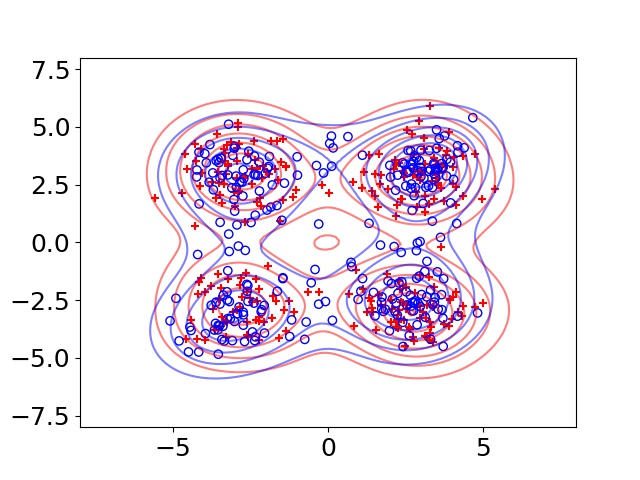
\includegraphics[width=0.3\linewidth]{images/toy/gauss4/frame12.jpg}
                                                                     %                                                                      \label{fig-toy1}
                                                                     %                                                                      }
                                                                     %                                                                      \centering
                                                                     %                                                                      \subfigure[$9$ Gaussians (standard deviation $1$).]
                                                                     %                                                                      {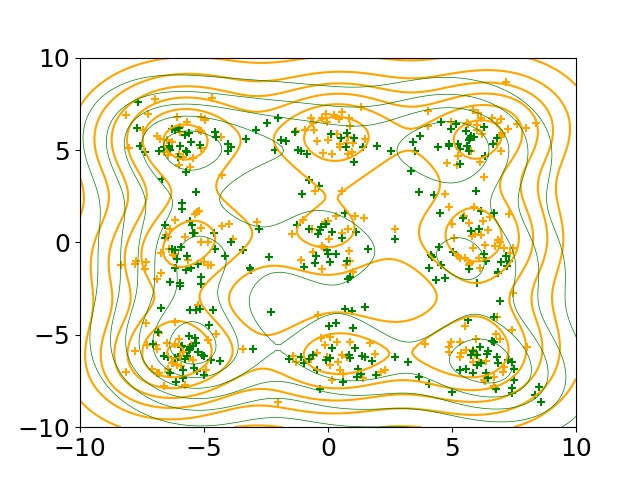
\includegraphics[width=0.3\linewidth]{images/toy/gauss9/frame11.jpg}
                                                                     %                                                                      \label{fig-toy2}
                                                                     %                                                                      }
                                                                     %                                                                      \centering
                                                                     %                                                                      \subfigure[Swissroll with Gaussian noise (standard deviation $2/3$).]
                                                                     %                                                                      {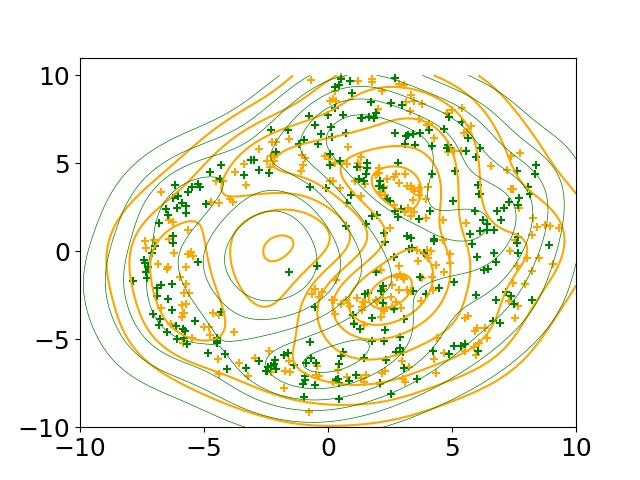
\includegraphics[width=0.3\linewidth]{images/toy/swiss/frame10.jpg}
                                                                     %                                                                      \label{fig-toy3}
                                                                     %                                                                      }
                                                                     %                                                                      \caption{Toy distribution learning: mixture Gaussian and
                                                                     %                                                                      Swissroll. A new batch of empirical samples of size $256$ are
                                                                     %                                                                      drawn in each iteration. Real samples (orange '+') and contour
                                                                     %                                                                      (orange curve), versus generated samples (green '+') by $g$ contour
                                                                     %                                                                      (green curve). 
                                                                     %                                                                      }\label{fig-toy}
                                                                     %                                                                      \end{figure}


                                                                     %                                                                      \begin{figure}[t!]
                                                                     %                                                                      \centering
                                                                     %                                                                      \subfigure[Empirical samples from Cifar10 dataset]
                                                                     %                                                                      {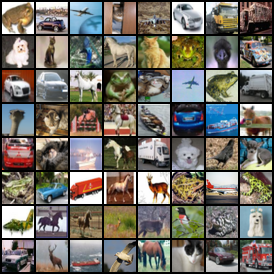
\includegraphics[width=0.45\linewidth]{images/cifar_hard/real_samples_19500.png}}
                                                                     %                                                                      \subfigure[Generated samples by $gf$ using loss defined in
                                                                     %                                                                      \eqref{eq-entropic-wsd}]
                                                                     %                                                                      {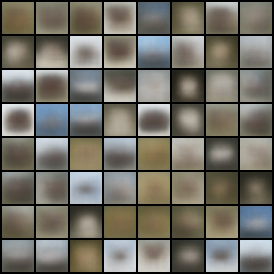
\includegraphics[width=0.45\linewidth]{images/cifar_hard/fake_samples_19500.png}}
                                                                     %                                                                      \caption{Blur samples generated by $g$ via loss defined in
                                                                     %                                                                      \eqref{eq-entropic-wsd} on Cifar10}\label{fig-wsd}
                                                                     %                                                                      \end{figure}
\subsection{Evaluation of generative models using MNIST}
In this subsection we evaluate both the generative models using MNIST dataset.
The representation mapping $\bm{f}$ in EOTGAN adapts two converlutional layers
appended with fully connected layers\footnote{$32$ Conv2d $5 \times5$
  $\rightarrow$ PReLU $\rightarrow$ MaxPool $2\times2$ $\rightarrow$
  $64$ Conv2d $5\times5$ $\rightarrow$ PReLU $\rightarrow$ MaxPool
  $2\times2$ $\rightarrow$ Dense $256$ $\rightarrow$ PReLU
  $\rightarrow$ Dense $256$ $\rightarrow$ PReLU $\rightarrow$ Dense
  $2$}
similar to \cite{1467314}\cite{1640964}. Generator $\bm{g}$ uses the same
setting as that of DCGAN and WGAN. Noise $P_z$ is $100$-dimensional Guassian.
We report IS and FID scores of EOTGAN in comparison with DCGAN and WGAN. Since EOTGAN is trained with representation mapping $\bm{f}$ that
acts as feature mapping, it is not fair to use this representation mapping $\bm{f}$ to do the
evaluation and make comparison since it would gives EOTGAN
advantages. Similar to \cite{2018arXiv180607755X}, we train a 34-layer
ResNet on MNIST to perform feature extraction for metric measurements
of IS and FID. In addition, we put EOTGM (Algorithm~\autoref{algo-E-WL}) in the comparison as well.

Data for evaluations is constructed by mixing empirical samples and
synthetic samples generated by $\bm{g}$. We draw the set $\mathcal{S}_{\mathrm{em}}$ of 2000 empirical samples from MNIST dataset. To generate a set $\mathcal{S}_{\mathrm{syn}}$ of synthetic
samples we draw $2000r$ samples from the generator network $\bm{g}$ where
$r\in[0,1]$ while rest $2000(1-r)$ are sampled directly from
MNIST. All following experiments are applied on
$\mathcal{S}_{\mathrm{em}}$ and $\mathcal{S}_{\mathrm{syn}}$. 
The way of mixing empirical data and generated data helps
us to identify if a metric is intuitively helpful. Among the chosen metrics IS at $r=0$ serves as a upper bound for the test while the FID at $r=0$ serves as a lower bound for the corresponding tests. %, and they should not decrease with the increase of $r=0$. Any results that breaking these rules may denote invalidity of a metric..

IS measures how certain a classifier assigns a class label to a given
generated sample. The larger IS is, the better the generative model
is. We plot IS versus $r$ for different models in
Fig. \ref{fig-tra-is}. IS scores of all four tested models drop with
increasing portion of synthetic samples in
$\mathcal{S}_{\mathrm{syn}}$, which is consistent with intuition. IS
of EOTGAN drops at the slowest rate among the four model as more
synthetic samples, for larger $r$, are mixed into test data. It shows
that EOTGAN outperforms WGAN and DCGAN in this test. EOTGM is found to provide the lowest IS.
This may be attributed to the setup that 
EOT optimization with cost measured by Euclidean distance of signals
fails to capture semantic similarity.
%Though \cite{2018arXiv180607755X}, \cite{2018arXiv180101973B} claimed
%that IS should not be used on dataset beyond ImageNet, the results
%in Fig.~\ref{fig-tra-is} is based on the ResNet that we have trained
%on MNIST and thus can be used for the classification in IS metric.

In Fig.~\ref{fig-tra-fid} the perfomances of different models are
compared using the FID metric. The smaller the FID of a generative model is, the more similar the
generated samples are to the empirical samples. EOTGAN is the least affected model among all the four, as the ratio $r$ increases, i.e. the generated samples by EOTGAN is more similar to the empirical
ones in the feature space regarding to FID. FID of WGAN is larger than that of EOTGAN. As
more generated samples are mixed the FIDs of DCGAN and EOTGM grow
even faster, which means the samples generated by these two models are
less similar to the empirical samples.
\section{Summary}
This work shows that entropy-regularized optimal transport cost is
useful to train neural network based generative models for learning implicit probability
distributions. With computationally efficient Sinkhorn algorithm,
learning of a probability distribution by a generative model can be
posed as an one-shot optimization problem. For further progress in
quality of generating samples, our experiments show that additional use of
representation mapping and alternative optimization based on
adversarial game produce better
semantic samples. 


\section{Related Work}


\subsection{Base: Generative Adversarial Network}


\subsection{Siamese Structure and Triplet Loss}

Siamese architecture is commonly used in verification or
authentication learning problems\cite{1467314}, which always take a
pair of inputs $x_1, x_2$ that are mapped by same $f: \Xx \rightarrow
\Mm$, the output "energy" $\norm{f(x_1) - f(x_2)}$ measures the
compatibility/similarity for the pair of inputs.
Triplet loss \cite{7298682} takes triple inputs: $x_1, x_2, y \in \Xx$
that are anchor, positive and negative input respectively and try to
learn $\bm{f}$ such that positive inputs always has smaller "energy" than
the negative inputs with regarding to anchor inputs,
$\normd{f(x_1)-f(x_2)}^2 + \gamma \le \normd{f(x_1)-f(y)}^2$, 
where $\gamma$ is margin value.

% The anchor and positive inputs are chosen in same class
% and $Y$ from a different class. Embedding $f$
% functions as if a "similarity" metric, after mapping of which
% distance of anchor and positive is minimized, while the distance of
% anchor and negative is maximized. The triplet loss is defined
% \cite{7298682}
% \begin{equation}
%     \sum_{i}^{N}\left[\normd{f(x_1^{(i)})-f(x_2^{(i)})}^2 - 
%     \normd{f(x_1^{(i)})-f(y^{(i)})}^2 + \ga \right]_{+},
% \end{equation}
% where $[\cdot]_{+} = \max(0, \cdot)$. 

Recent work \cite{2017arXiv171105084C} has proposed 
the TripletGAN that is close research to
our work, where the generative model is trained by solving the
following minimax problem:
\begin{equation}
  \min_{g} \max_{f} \EE_{{\substack{X\sim P \\ Y_1= g(Z_1)\\ Y_2 = g(Z_2)}}}\left[ \normd{f(Y_1)-f(X)}^2 - \normd{f(Y_1)-f(Y_2)}^2 \right],
\end{equation}
where $Z_1, Z_2 \sim P_z$ and $(Z_1,Z_2,X)$ are mutually independent. The TripletGAN has two virtual
"classes" no matter how many the empirical dataset actually has. It treats samples
$X\sim P$ from empirical dataset as if a virtual positive "class" while the all
generated samples $Y=g(Z), Z\sim P_z$ as a negative "class". 

\section{Summary}
\section{Raw}
\section{Introduction}

Data-driven learning of a probability distribution by a generative model is an important problem 
in statistical signal processing and machine learning. 
Recently neural network based generative models are popular tools to
study underlying probability distribution of datasets. A prominent example is 
generative adversarial network (GAN) \cite{NIPS2014_5423}, which learns 
implicit distribution models. 

In the GAN of \cite{NIPS2014_5423}, a generator produces
synthetic samples and a discriminator endeavors to
distinguish between real samples and synthetic samples. Generators and discriminators are realized using (deep) neural networks.
Discriminator and generator
play an adversary game against each other using a `min-max' optimization to learn parameters of neural networks. 
For generator, the game
turns out be minimizing Jensen-Shannon divergence (JSD) between
target distribution and induced distribution by generator when discriminator is
optimal. Using the same adversary
optimization, deep convolutional neural network based GAN (DCGAN)
\cite{2015arXiv151106434R} producing good quality synthetic images, has attracted high attention.

JSD has limitations in GANs where generators and dis-
criminators are based on deep neural networks. The first limitation is that back
propagation suffers from vanishing gradient. Gradient of cost
function with respect to (w.r.t.) generator vanishes as
discriminator approaches optimal (see Theorem~2.4~\cite{2017arXiv170104862A}),
which stops generator from further learning. The second limitation is due to high sensitivity of JSD to slight perturbations. JSD can be large between a distribution $P_x$ and a distribution $P_{x+\epsilon}$ where $\epsilon$ is perturbation\cite{2017arXiv170104862A}. 

Both limitations are addressed in Wasserstein GAN (WGAN)
\cite{2017arXiv170107875A}. Wasserstein distance stems from
optimal transport (OT) problem, which measures divergence between two
distributions. The WGAN formulation does not require an explicit
discriminator and it does not has the vanishing-gradient problem. Further,
Wasserstein distance/OT is upper bounded by the standard deviation of perturbation $\epsilon$
\cite{2017arXiv170104862A}, addressing the second limitation. 

OT based cost in WGAN brings a strict constraint to follow in its optimization.
Kantorovich-Rubinstein duality used in WGAN requires a supremum over
infinite set of all Lipschitz functions with Lipschitz constant equal
to one. Various sub-optimal techniques are proposed to enforce the
Lipschitz property. An example is weight clipping
\cite{2017arXiv170107875A} where neural network parameters (weights)
are updated first without Lipschitz constraint and then projected to
satisfy Lipschitz constraint in each iteration. Other approaches are
gradient penalty\cite{2017arXiv170400028G} and spectrum normalization\cite{2018arXiv180205957M}.

In this article, our main contribution is to explore use of Entropy-regularized OT (EOT) cost for generative models. 
The EOT was studied earlier for efficient comparison between two probability distributions \cite{2013arXiv1306.0895C}. 
The major advantage of EOT is
that corresponding dual problem is free from Lipschitz constraint. Use of EOT improves
analytical tractability allows us to develop two generative models. Our
first model considers EOT cost directly on distribution of signals (in our case,
on the image pixels). This model uses an one-shot optimization problem, \emph{i.e.} no use of adversarial game in iterations. The second model
considers EOT on feature distribution instead of direct signal
distribution. In this case we also need to learn a representation
mapping, which is implemented as a neural network. 
This requires alternative optimization of representation mapping and
generator. In addition to the above advantage, duality of EOT can be
effectively solved and straightforwardly extended to parallel computation. 





% However, Pixel representation of images does not induce meaningful
% Euclidean distances\cite{ponce2011computer}. Thus applying Algorithm~\ref{algo-E-WL}
% directly in $\Xx$ for problem in \eqref{eq-entropic-wsd} may not
% guide $g$ to generate meaningfully semantic samples.
% Assuming there is feature mapping for samples, then we
% can apply Algorithm~\ref{algo-E-WL} in the feature domain to avoid the
% above problem. To measure how semantically similar two
% samples are, we define a similarity metric
% 
% \begin{equation}\label{def-similarity}
%   d_f(y, x) \coloneqq \|f(y)-f(x)\|_{2,\mathcal{M}}^{2}.
% \end{equation}
% where $f: \Xx \rightarrow \Mm$, $\mathcal{M}\subset\mathbb{R}^{m}$, which is
% parameterized by $\omega$, $\|\cdot\|_{2,\mathcal{M}}^{2}$ is the
% corresponding squared Euclidean distance in feature space $\Mm$.
% $f$ here maps the input patterns into the feature space $\Mm$ where
% semantic distance is approximated. Since $f$ takes values in $\Xx$,
% we try to learn a push-forward probability distribution $P$ in feature space $\Mm$, instead of
% learning in $\Xx$ to avoid the instability problem of approximating
% distribution in high-dimension domain.
% 
% However, $f$ usually is dataset-dependent. In order to get $f$ we use
% triple loss to learn $f$ in \eqref{def-similarity}. We
% assume samples from $P$ belong to positive class, and samples from
% $g$'s induced distribution $Q$ belong to negative class. Samples from
% same class share common features and should have small OT distance in
% feature domain $\Mm$, while OT distance between different classes
% should be large in $\Mm$. Then learning of $f$ is minimizing:
% \begin{equation}\label{eq-sim-in}
%   W_f(P, P) = \inf_{\pi_{\mathrm{in}} \in \Pi(P, P) }\dotp{\pi_{\mathrm{in}}}{M_{\mathrm{in}}} - \la H(\pi_{\mathrm{in}}),
% \end{equation}
% where $[M_{\mathrm{in}}]_{i,j} = d_f(x_i, \tilde{x}_j), x_i,
% \tilde{x}_j \sim P$, while maximizing:
% \begin{equation}\label{eq-sim-ex}
%   W_f(P, Q) = \inf_{\pi_{\mathrm{ex}} \in \Pi(P, Q) }\dotp{\pi_{\mathrm{ex}}}{M_{\mathrm{ex}}} - \la H(\pi_{\mathrm{ex}}),
% \end{equation}
% where $[M_{\mathrm{ex}}]_{i,j} = d_f(x_i, y_j)$, $x_i \sim P, y_j\sim
% Q$. Note \eqref{eq-sim-in} makes sense since two different random batchs of
% samples from $P$ are used for large datasets.
% 
% 
% Since both $W_f(P, P)$ and $W_f(P, Q)$ are
% lowered bounded instead of upper bounded, similar to triplet loss used
% in \cite{7298682}, feature mapping $f$ here is trained by minimizing a hinge loss
% $\Ll_{f}(P, Q)$ while generator $g$ is trained by adversarially
% minimizing $\Ll_{g}(P, Q)$, EOT distance between empirical and synthetic
% samples:
% \begin{align}
    %     \Ll_f(P, Q) &= \max\left(0, W_f(P,P)- W_f(P,Q) + \gamma \right),
                        %                         \nonumber \\
    %     \Ll_g(P,Q) &= W_f(P,Q).
                       %   \end{align}
                       %                        where $\gamma>0$. Hinge adversarial loss here helps to balance the adversarial
                       %                        training of the $f$ and $g$.
                       %                        Note the our hinge adversarial loss shares similarity only in form to the self-attention
                       %                        GAN\cite{2018arXiv180508318Z} and geometric GAN\cite{2017arXiv170502894L}
                       %                        but is motivated differently and defined in different metric.
                       %                        
                       %                        Then the adversarial training between similarity mapping $f$ and
                       %                        generator $g$ is alternatively minimizing:
                       %                        \begin{align}
                       %                      &\min_{f} \Ll_f(P, Q) = \min_{\omega} \Ll_f(P, Q)\nonumber \\
    %                       &\min_{g} \Ll_g(P, Q) = \min_{\th} \Ll_{g}(P, Q)
                              %   \end{align}
                              %                               where $\omega$ is parameter of $f$. This is an
                              %                               adversarial optimization approach using the EOT discussed in
                              %                               Subsection \ref{subsec-gmeot}. We refer it as EOTGAN whose algorithm is summarized in Algorithm \ref{algo-eWGAN}.


                              %                               Other techniques may be
                              %                               used to even further to reduce the computation complexity bellow $\mathcal{O}(N^2)$\cite{2018arXiv180300567P}.

                              %                               \textcolor{red}{We need to show Lipschitz form and what are the problems}

                              %                               \subsection{Entropy-constrained  OT cost}

                              %                               \subsection{Entropy-constrained OT GAN}


                              %                               \subsection{Entropy-regularized OT}\label{subsec-wsd}

                              %                               To relieve the computation burden, we are going to apply entropic
                              %                               regulation to the original objective function of OT and employ the
                              %                               Sinkhorn algorithm \cite{2013arXiv1306.0895C} for fast computation,
                              %                               which provides accurate and stable computation, and can
                              %                               be well parallelized on GPU execution. Additionally, the entropy
                              %                               regularization allows smooth solution to the OT problem.
                              %                               The Entropy-regularized OT (EOT) can be formulated as:
                              %                               \begin{equation}
                              %                               W(P,Q)=\min_{\pi\in \Pi(P,Q)} \dotp{\pi}{M} - \la H(\pi),
                              %                               \end{equation}
                              %                               where $[M]_{i,j} = d(x_i, y_j) = \normd{x_i - y_j}$ and $x_i, y_j$ are
                              %                               samples of $P, Q$ respectively, $H(\pi) = \sum_{i,j} -\pi_{i,j}
                              %                               \log(\pi_{i,j})$ and $\la \in \RR^{+}$ is the regulation parameter.
                              %                               Using duality, the EOT problem can be formulated as
                              %                               \begin{equation}
                              %                               W(P,Q) = \max_{\al, \be \in \mathbb{R}^{N}} \al^{T}P + \beta^{T}Q -
                              %                               \sum_{i,j} \lambda e^{ {\left( \al + \beta - [M]_{i,j} \right)}/{\la} }
                              %                               \end{equation}

                              % %                               \begin{prop}
                              % %                                 \unsure{Minh, any analysis you want to put here? For the proposition?}
                              % %                                 Let generator $g: \Zz \rightarrow \Xx$ be parameterized by $\th \in \Theta$
                              % %                                 and $g$ is differentiable w.r.t $\th$. The subgradient of the entropy
                              % %                                 regularized Wasserstain distance loss with respect to parameter of
                              % %                                 generator $G$ is:
                              % %                                 \begin{equation}
                              % %                                   \pd{J(Q, P)}{\th} = (\pd{G}{\th})^{T} \alpha,
                              % %                                 \end{equation}
                              % %                                 where $\al$ is obtained by the following sinkhorn algorithm:

                              % %                                 \begin{algorithm}
                              % %                                   \caption{Computation of Entropy Regularized Wasserstein Loss}\label{algo-sinkhorn}
                              % %                                   \begin{algorithmic}[1]
                              % %                                     \Require{$M, \la, p, q$ \Comment{$p,q$ lies in probability simplex
                              % %                                     for distribution $P, Q$.\\ $M_{i,j} = d(x_i, y_j)$ }}
                              % %                                     \State $K = \exp(-M/\la)$
                              % %                                     \State $x = ones(length(q))/length(q)$
                              % %                                     \While{$x$ not converge}
                              % %                                     \State $x \gets diag(1/q)*K*(p*(1./(K^{T}1./q)) $
                              % %                                     \EndWhile\label{euclidendwhile}

                              % %                                     \State $u \gets 1./x, v \gets q.*(1./K^{T}*u)$
                              % %                                     \State $\pi \gets \mathrm{diag}(u)K \mathrm{diag}(v)$
                              % %                                     \State $\al \gets -\la \log(u) + \la \ones^{T} \log(u)/length(q)*\ones$

                              % %                                   \end{algorithmic}
                              % %                                 \end{algorithm}
                              % %                               \end{prop}


    %     The optimal dual vector $\beta^{\ast}$
    %     of \eqref{eq-dual-opt} is
    %     actually a subgradient of $W(P,Q)$ w.r.t. $Q$. $\beta^{\ast}$ can be efficiently
    %     computed by alternatively scaling the rows and columns of $M$ by
    %     Sinkhorn algorithm\cite{2013arXiv1306.0895C, 2013arXiv1310.4375C}
    %     , which gives a pair of
    %     vectors $(u, v) \in \RR^n_{+} \times \RR^m_{+}$ that define the
    %     optimal primary and dual arguments: $\pi^{\ast} =
    %     \mathrm{diag}(u)e^{-M/\la}\mathrm{diag}(v), \beta^{\ast} = -\frac{\log(u)}{\la} +
    %     \frac{\log(u)\mathds{1}_n}{n\la} \mathds{1}_n$.


    % %     We show by a toy dataset in Subsection \ref{subsec-mg}, solving problem
    % %     \eqref{eq-entropic-wsd} gives the distribution $Q$ represented by
    % %     generator $g$, which is close to empirical distribution $P$. %According to
    % %     \cite{2017arXiv170107875A}, the convergence of OT distance
    % %     between $Q$ and $P$ guarantees their $KL$ divergence, i.e. $T(P,Q)
    % %     \rightarrow 0$ implies $KL(P \| Q) \rightarrow 0$.



    %     \input{section/sec-entropy-wgan}
    %     \input{section/sec-experimental}



%%% Local Variables:
%%% mode: latex
%%% TeX-master: "../../main"
%%% End:
